
\section{Higher-Order Momentum Balance}
\label{sc:higher-order-mom}

\begin{figure}
  \begin{center}
    \includegraphics[width=0.65\columnwidth]{\dir/figs/GIS.eps}
   \end{center}
  \caption{Observation-based balance velocities for Greenland (left) and depth-averaged speed from higher-order CISM (right) with basal sliding coefficients optimized to match the balance velocities (after Price et al., $PNAS$, \textbf{108}(22), 2011).}
  \label{fig:GIS_PNAS}
\end{figure} 

The higher-order dynamics scheme in CISM (some output from which is shown in Figure \ref{fig:GIS_PNAS}) is discussed in more detail in the following sections. 
First we describe the derivation of the equations themselves, followed by a discussion and derivation of the boundary conditions.
We then describe generic solution methods for the nonlinear system of equations, followed by a
brief discussion of the solution of the thickness evolution equation.

% Commented out the subsection because there are no other subsections in this section
%\subsection{Derivation of the Blatter-Pattyn Equations}
%\label{sc:higher-order-blatter-pattyn}

The higher-order dynamics scheme in CISM is based on the 3d first-order accurate Stokes approximation (also often referred to as the ``Blatter-Pattyn" model). The starting point is the nonlinear Stokes equations:

\begin{equation}
  \begin{split}
    & x:\quad \frac{\partial \tau _{xx}}{\partial x} + \frac{\partial \tau _{xy}}{\partial y} + \frac{\partial \tau _{xz}}{\partial z} - \frac{\partial P}{\partial x} = 0, \\ 
    & y:\quad \frac{\partial \tau _{xy}}{\partial x} + \frac{\partial \tau _{yy}}{\partial y} + \frac{\partial \tau _{yz}}{\partial z} - \frac{\partial P}{\partial y} = 0, \\ 
    & z:\quad \frac{\partial \tau _{xz}}{\partial x} + \frac{\partial \tau _{zy}}{\partial y} + \frac{\partial \tau _{zz}}{\partial z} - \frac{\partial P}{\partial z} = \rho_i g,
  \end{split}
\end{equation}

\noindent
where \textit{P} is the pressure and {\large \(\tau{}\)} is the deviatoric stress tensor. The latter is given by $\tau _{ij}=\sigma _{ij}+P\delta _{ij}$, 
where {\large \(\sigma{}\)} is the full stress tensor.

There are a number of ways to argue that, due to the shallowness of ice sheets (i.e., the small value of \textit{H}/\textit{L}, where \textit{H} is the thickness and \textit{L} is a relevant horizontal length scale), the Stokes equations can be reduced to the following first-order approximation:

\begin{equation}
  \begin{split}
    & x:\quad \frac{\partial \tau _{xx}}{\partial x} + \frac{\partial \tau _{xy}}{\partial y} + \frac{\partial \tau _{xz}}{\partial z} - \frac{\partial P}{\partial x} = 0, \\ 
    & y:\quad \frac{\partial \tau _{yy}}{\partial y} + \frac{\partial \tau _{xy}}{\partial x} + \frac{\partial \tau _{yz}}{\partial z} - \frac{\partial P}{\partial y} = 0, \\ 
    & z:\quad \frac{\partial \tau _{zz}}{\partial z} - \frac{\partial P}{\partial z} = \rho g. \\ 
  \end{split}
\end{equation}

\noindent
The arguments supporting this reduction are fairly complex and are based on either a variational analysis or an asymptotic analysis (see \citet{Schoof:2010dl} and \citet{DUKOWICZ:2010wb} for details).

The third (vertical) balance equation above can be integrated vertically to give an expression for the pressure:
\begin{equation}
P = \rho g\left( s-z \right) + \tau _{zz}(z).
\end{equation} 
This is simply a statement that the full vertical normal stress is balanced by the hydrostatic pressure (the so-called \textit{hydrostatic assumption}). This expression can be substituted into the horizontal pressure gradient terms above to remove pressure from the equations. For example, for the \textit{x} component of velocity we have

\begin{equation}
  \label{ho.eq.x_stress_balance}
  \begin{split}
    & \frac{\partial \tau _{xx}}{\partial x} + \frac{\partial \tau _{xy}}{\partial y} + \frac{\partial \tau _{xz}}{\partial z} = \frac{\partial }{\partial x}\left[ \rho g\left( s-z \right)+\tau _{zz}(z) \right] \\ 
    & \frac{\partial \tau _{xx}}{\partial x} - \frac{\partial \tau _{zz}}{\partial x} + \frac{\partial \tau _{xy}}{\partial y} + \frac{\partial \tau _{xz}}{\partial z} = \rho g\frac{\partial s}{\partial x} \\ 
  \end{split}
\end{equation}

\noindent
Using the incompressibility constraint \eqref{ho.eq.incompress} and the assumption that stress and strain are aligned we can write

\begin{equation}
  \label{ho.eq.incompress_tau}
  \tau _{zz} = -\tau _{xx}-\tau _{yy}.
\end{equation}

\noindent
Taking the gradient of \eqref{ho.eq.incompress_tau} with respect to $x$, we can rewrite the vertical normal deviatoric stress in terms of horizontal normal deviatoric stresses:

\begin{equation}
  \label{ho.eq.incompress_tau_dx}
  -\frac{\partial \tau _{zz}}{\partial x} = -\frac{\partial }{\partial x}\left( -\tau _{xx} - \tau _{yy} \right) = \frac{\partial \tau _{xx}}{\partial x} + \frac{\partial \tau _{yy}}{\partial x}.
\end{equation}
 
\noindent
Substituting \eqref{ho.eq.incompress_tau_dx} into \eqref{ho.eq.x_stress_balance}, we obtain
 
\begin{equation}
%  2\frac{\partial \tau _{xx}}{\partial x} + \frac{\partial \tau _{yy}}{\partial x} + \frac{\partial \tau _{xy}}{\partial y} + \frac{\partial \tau _{xz}}{\partial z} = \rho g\frac{\partial s}{\partial x}.
  \label{ho.eq.stress_balance_x}
  \frac{\partial }{\partial x} \left( 2 \tau_{xx} + \tau_{yy} \right) + \frac{\partial \tau _{xy}}{\partial y} + \frac{\partial \tau _{xz}}{\partial z} = \rho g\frac{\partial s}{\partial x}.
\end{equation}

\noindent
Similarly, the $y$ horizontal balance equation is
\begin{equation}
  \label{ho.eq.stress_balance_y}
  \frac{\partial }{\partial y} \left( 2 \tau_{yy} + \tau_{xx} \right) + \frac{\partial \tau _{xy}}{\partial x} + \frac{\partial \tau _{yz}}{\partial z} = \rho g\frac{\partial s}{\partial y}.
\end{equation}

\noindent 
At this point we have removed the vertical balance equation entirely; it has been incorporated into the horizontal balance equations through incompressibility.


%\begin{align*}
%  & x:\quad 2\frac{\partial \tau _{xx}}{\partial x}+\frac{\partial \tau _{yy}}{\partial x}+\frac{\partial \tau _{xy}}{\partial y}+\frac{\partial \tau _{xz}}{\partial z}=\rho g\frac{\partial s}{\partial x}\quad,  \\ 
% & y:\quad 2\frac{\partial \tau _{yy}}{\partial y}+\frac{\partial \tau _{xx}}{\partial y}+\frac{\partial \tau _{xy}}{\partial x}+\frac{\partial \tau _{yz}}{\partial z}=\rho g\frac{\partial s}{\partial y}. \\
%\end{align*}

Next we want to write these equations in terms of the velocities for which we are ultimately solving. Stresses and velocities are linked through the 
constitutive law for ice, which relates strain rates to stresses (here we assume Nye's generalization of Glen's law), and through the 
definition of the strain rate tensor, which relates strain rates to velocity gradients:

\begin{equation}
  \begin{split}
    & 1.\quad \tau _{ij}=B\dot{\varepsilon }_{e}^{\frac{1-n}{n}}\dot{\varepsilon }_{ij},\quad B=B(T) \\ 
    & 2.\quad \dot{\varepsilon }_{ij}=\frac{1}{2}\left( \frac{\partial u_{i}}{\partial x_{j}}+\frac{\partial u_{j}}{\partial x_{i}} \right) \\ 
    & 3.\quad 2\dot{\varepsilon }_{e}=\dot{\varepsilon }_{ij}\dot{\varepsilon }_{ij} \\ 
    & 4.\quad \eta \equiv \frac{1}{2}B\dot{\varepsilon }_{e}^{\frac{1-n}{n}} \\ 
    & 5.\quad \tau _{ij}=2\eta \dot{\varepsilon }_{ij} \\ 
  \end{split}
\end{equation}

\noindent
In order, the five expressions above give: 

\begin{enumerate}
\item  Glen's flow law\footnote{Technically, we are using the \textit{inverse} form of the flow-law here.}, where 
$B = A^{\frac{-1}{n}}$ is the temperature dependent rate factor 
\item  The definition of the strain-rate tensor in terms of velocity gradients
\item  The definition of the effective strain rate, $\dot{\varepsilon }_{e}$, a norm of the strain-rate tensor
\item  A definition of the ``effective viscosity" (after rearranging some terms in (1))
\item  Items (1)-(4) allow us to write the relationship between stress and strain in a standard ``Newtonian" way, but with a non-Newtonian (nonlinear) viscosity
\end{enumerate}

\noindent
Now, taking these definitions into the stress balance equations \eqref{ho.eq.stress_balance_x} and \eqref{ho.eq.stress_balance_y} 
and expanding in terms of strain rates and effective viscosity, we have (for the \textit{x} direction only):

\begin{equation}
  x: \quad 2\frac{\partial }{\partial x}\left( 2\eta \dot{\varepsilon }_{xx} \right) + \frac{\partial }{\partial x}\left( 2\eta \dot{\varepsilon }_{yy
} \right) + \frac{\partial }{\partial y}\left( 2\eta \dot{\varepsilon }_{xy} \right) + \frac{\partial }{\partial z}\left( 2\eta \dot{\varepsilon }_{xz} 
\right) = \rho g\frac{\partial s}{\partial x}, \\ 
%  x: \quad 2\frac{\partial }{\partial x} \left( 2\eta \dot{\varepsilon }_{xx} +  2\eta \dot{\varepsilon}_{yy} \right) +\frac{\partial }{\partial y}\left( 2\eta \dot{\varepsilon }_{xy} \right)+\frac{\partial }{\partial z}\left( 2\eta \dot{\varepsilon }_{xz} \right)=\rho g\frac{\partial s}{\partial x}. \\ 
\end{equation}

\noindent
Replacing strain-rate components with velocity gradients, we obtain

\begin{equation}
  \label{ho.eq.stress_balance_final_x}
  x: \quad \frac{\partial }{\partial x}\left( 4 \eta \frac{\partial u}{\partial x} +  2 \eta \frac{\partial v}{\partial y} \right) + \frac{\partial }{\partial y}\left[ \eta \left( \frac{\partial u}{\partial y} + \frac{\partial v}{\partial x} \right) \right]+\frac{\partial }{\partial z}\left( \eta \frac{\partial u}{\partial z} \right) = \rho g\frac{\partial s}{\partial x}.
\end{equation}

\noindent
An analogous expression gives the \textit{y}-direction momentum balance: 

\begin{equation}
  \label{ho.eq.stress_balance_final_y}
  y: \quad \frac{\partial }{\partial y}\left( 4 \eta \frac{\partial v}{\partial y} +  2 \eta \frac{\partial u}{\partial x} \right) + \frac{\partial }{\partial x}\left[ \eta \left( \frac{\partial u}{\partial y} + \frac{\partial v}{\partial x} \right) \right]+\frac{\partial }{\partial z}\left( \eta \frac{\partial v}{\partial z} \right) = \rho g\frac{\partial s}{\partial y}.  
\end{equation}

\noindent
These are the basic equations to be discretized and solved.

%Thus, the final form of the equations to be discretized and solved is given by:

%\begin{align*}
%  & x:\quad 4\frac{\partial }{\partial x}\left( \eta \frac{\partial u}{\partial x} \right)+\frac{\partial }{\partial y}\left( \eta \frac{\partial u}{\partial y} \right)
%  +2\frac{\partial }{\partial x}\left( \eta \frac{\partial v}{\partial y} \right)+\frac{\partial }{\partial y}\left( \eta \frac{\partial v}{\partial x} \right)
%  +\frac{\partial }{\partial z}\left( \eta \frac{\partial u}{\partial z} \right)=\rho g\frac{\partial s}{\partial x}, \\ 
% & y:\quad 4\frac{\partial }{\partial y}\left( \eta \frac{\partial v}{\partial y} \right)+\frac{\partial }{\partial x}\left( \eta \frac{\partial v}{\partial x} \right)
% +2\frac{\partial }{\partial y}\left( \eta \frac{\partial u}{\partial x} \right)+\frac{\partial }{\partial x}\left( \eta \frac{\partial u}{\partial y} \right)
% +\frac{\partial }{\partial z}\left( \eta \frac{\partial v}{\partial z} \right)=\rho g\frac{\partial s}{\partial y}. \\ 
%\end{align*}
